% \documentclass[output=paper,
% modfonts
% ]{langscibook} 
% \bibliography{localbibliography}

% %\usepackage{tabularx,multicol}
\usepackage{url}
\urlstyle{same}

\usepackage{longtable} % to be able to make the long table in Data span over multiple pages - JP
\usepackage{multirow} % to be able to use the multirow command - needed for Paper 2 tables

\usepackage{langsci-lgr}
\usepackage{langsci-branding}
\usepackage{langsci-optional}
\usepackage{langsci-gb4e}


% %\makeatletter
\let\thetitle\@title
\let\theauthor\@author
\makeatother

\newcommand{\togglepaper}[1][0]{
%   \bibliography{../localbibliography}
  \papernote{\scriptsize\normalfont
    \theauthor.
    \thetitle.
    To appear in:
    Change Volume Editor \& in localcommands.tex
    Change volume title in localcommands.tex
    Berlin: Language Science Press. [preliminary page numbering]
  }
  \pagenumbering{roman}
  \setcounter{chapter}{#1}
  \addtocounter{chapter}{-1}
}

\newcommand{\bari}{\ipabar{\i}{.5ex}{1.1}{}{}}
\newcommand{\notipa}[1]{\textnormal{#1}}

\newcommand{\agre}{\textsc{agr}-\ol{eene}}

\renewcommand{\emph}[1]{\textit{#1}} % resetting a setting from ling-macros-modified (I think?)

% forest settings to make compact but (mostly) straight-spined trees:
\forestset{
fairly nice empty nodes/.style={
            delay={where content={}{shape=coordinate,for parent={
                  for children={anchor=north}}}{}}
, angled/.style={content/.expanded={$<$\forestov{content}$>$}}
}}

\forestset{sn edges/.style={for tree={parent anchor=south, child anchor=north}}}

\newcommand{\bex}{\begin{exe}}
\newcommand{\fex}{\end{exe}}

\newcommand{\bxl}{\begin{exe}}
\newcommand{\fxl}{\end{exe}}

\newcommand{\ix}[1]{\textsubscript{#1}}
\newcommand{\alert}[1]{\textbf{#1}}
\newcommand{\ol}[1]{\textit{#1}}


\newenvironment{context}{\begin{quote}%
			\bfseries Context: \\%
			\mdseries\slshape }%open environment
			{\end{quote}}%close environment




			\usetikzlibrary{shapes,arrows,positioning,decorations,decorations.pathmorphing,intersections}
\forestset{
nice empty nodes/.style={
    for tree={calign=fixed edge angles},
    delay={where content={}{shape=coordinate,for siblings={anchor=north}}{}}
},
}

\definecolor{dark-gray}{gray}{0.3}

%\usepackage{dingbat,pifont}


%%%%%%%%%%%%For arrows%%%%%%%%%%%%%

\newcommand\Tikzmark[2]{%
  \tikz[remember picture]\node[inner sep=0pt,outer sep=0pt] (#1) {#2};%
}
\NewDocumentCommand\DrawArrow{O{}mmmmO{3}}{
\tikz[remember picture,overlay]
  \draw[->,line width=0.8pt,shorten >= 2pt,shorten <= 2pt,#1]
    (#2) -- ++(0,-#6\ht\strutbox) coordinate (aux) -- node[#4] {#5} (#3|-aux) -- (#3);
}
\NewDocumentCommand\DrawDotted{O{}mmmmO{3}}{
\tikz[remember picture,overlay]
  \draw[->,line width=0.9pt,dotted,shorten >= 2pt,shorten <= 2pt,#1]
    (#2) -- ++(0,-#6\ht\strutbox) coordinate (aux) -- node[#4] {#5} (#3|-aux) -- (#3);
}
\NewDocumentCommand\DrawLine{O{}mmmmO{3}}{
\tikz[remember picture,overlay]
  \draw[line width=0.8pt,shorten >= 2pt,shorten <= 2pt,#1]
    (#2) -- ++(0,-#6\ht\strutbox) coordinate (aux) -- node[#4] {#5} (#3|-aux) -- (#3);
}
%%%%%%%%%%%%%%%%%%%%%%%%%%%%%%%%%%%%%


\newcommand{\baru}{ʉ}
\newcommand{\baruH}{\'\baru}
\newcommand{\baruL}{\`\baru}

\newcommand{\ep}{ε}
\newcommand{\epH}{\'\ep}
\newcommand{\epL}{\`\ep}

\newcommand{\schwa}{ə}
\newcommand{\schwaH}{\'ə}
\newcommand{\schwaL}{\`ə}

\newcommand{\oo}{ɔ}
\newcommand{\ooH}{\'\oo}
\newcommand{\ooL}{\`\oo}

\newcommand{\ds}{\ꜜ}

\newcommand{\ch}{t͡ʃ}
\newcommand{\dz}{d͡ʒ}

\newcommand{\tgl}{ʔ}

%shortcuts for the complementizers
\newcommand{\mbuL}{mb\baruL}
\newcommand{\mbuHL}{mb\baruH\baruL}
\newcommand{\mbuLH}{mb\baruL\baruH}
\newcommand{\la}{lá}
\newcommand{\nda}{ndà}

\newcommand{\tsc}[1]{\textsc{#1}}
\renewcommand{\textscb}{ʙ}
\newcommand{\ipa}[1]{#1} %disable IPA
 


% \IfFileExists{localcommands.tex}{
%  % \addbibresource{../localbibliography.bib}
% %  \usepackage{tabularx,multicol}
\usepackage{url}
\urlstyle{same}

\usepackage{longtable} % to be able to make the long table in Data span over multiple pages - JP
\usepackage{multirow} % to be able to use the multirow command - needed for Paper 2 tables

\usepackage{langsci-lgr}
\usepackage{langsci-branding}
\usepackage{langsci-optional}
\usepackage{langsci-gb4e}

% %  \makeatletter
\let\thetitle\@title
\let\theauthor\@author
\makeatother

\newcommand{\togglepaper}[1][0]{
%   \bibliography{../localbibliography}
  \papernote{\scriptsize\normalfont
    \theauthor.
    \thetitle.
    To appear in:
    Change Volume Editor \& in localcommands.tex
    Change volume title in localcommands.tex
    Berlin: Language Science Press. [preliminary page numbering]
  }
  \pagenumbering{roman}
  \setcounter{chapter}{#1}
  \addtocounter{chapter}{-1}
}

\newcommand{\bari}{\ipabar{\i}{.5ex}{1.1}{}{}}
\newcommand{\notipa}[1]{\textnormal{#1}}

\newcommand{\agre}{\textsc{agr}-\ol{eene}}

\renewcommand{\emph}[1]{\textit{#1}} % resetting a setting from ling-macros-modified (I think?)

% forest settings to make compact but (mostly) straight-spined trees:
\forestset{
fairly nice empty nodes/.style={
            delay={where content={}{shape=coordinate,for parent={
                  for children={anchor=north}}}{}}
, angled/.style={content/.expanded={$<$\forestov{content}$>$}}
}}

\forestset{sn edges/.style={for tree={parent anchor=south, child anchor=north}}}

\newcommand{\bex}{\begin{exe}}
\newcommand{\fex}{\end{exe}}

\newcommand{\bxl}{\begin{exe}}
\newcommand{\fxl}{\end{exe}}

\newcommand{\ix}[1]{\textsubscript{#1}}
\newcommand{\alert}[1]{\textbf{#1}}
\newcommand{\ol}[1]{\textit{#1}}


\newenvironment{context}{\begin{quote}%
			\bfseries Context: \\%
			\mdseries\slshape }%open environment
			{\end{quote}}%close environment




			\usetikzlibrary{shapes,arrows,positioning,decorations,decorations.pathmorphing,intersections}
\forestset{
nice empty nodes/.style={
    for tree={calign=fixed edge angles},
    delay={where content={}{shape=coordinate,for siblings={anchor=north}}{}}
},
}

\definecolor{dark-gray}{gray}{0.3}

%\usepackage{dingbat,pifont}


%%%%%%%%%%%%For arrows%%%%%%%%%%%%%

\newcommand\Tikzmark[2]{%
  \tikz[remember picture]\node[inner sep=0pt,outer sep=0pt] (#1) {#2};%
}
\NewDocumentCommand\DrawArrow{O{}mmmmO{3}}{
\tikz[remember picture,overlay]
  \draw[->,line width=0.8pt,shorten >= 2pt,shorten <= 2pt,#1]
    (#2) -- ++(0,-#6\ht\strutbox) coordinate (aux) -- node[#4] {#5} (#3|-aux) -- (#3);
}
\NewDocumentCommand\DrawDotted{O{}mmmmO{3}}{
\tikz[remember picture,overlay]
  \draw[->,line width=0.9pt,dotted,shorten >= 2pt,shorten <= 2pt,#1]
    (#2) -- ++(0,-#6\ht\strutbox) coordinate (aux) -- node[#4] {#5} (#3|-aux) -- (#3);
}
\NewDocumentCommand\DrawLine{O{}mmmmO{3}}{
\tikz[remember picture,overlay]
  \draw[line width=0.8pt,shorten >= 2pt,shorten <= 2pt,#1]
    (#2) -- ++(0,-#6\ht\strutbox) coordinate (aux) -- node[#4] {#5} (#3|-aux) -- (#3);
}
%%%%%%%%%%%%%%%%%%%%%%%%%%%%%%%%%%%%%


\newcommand{\baru}{ʉ}
\newcommand{\baruH}{\'\baru}
\newcommand{\baruL}{\`\baru}

\newcommand{\ep}{ε}
\newcommand{\epH}{\'\ep}
\newcommand{\epL}{\`\ep}

\newcommand{\schwa}{ə}
\newcommand{\schwaH}{\'ə}
\newcommand{\schwaL}{\`ə}

\newcommand{\oo}{ɔ}
\newcommand{\ooH}{\'\oo}
\newcommand{\ooL}{\`\oo}

\newcommand{\ds}{\ꜜ}

\newcommand{\ch}{t͡ʃ}
\newcommand{\dz}{d͡ʒ}

\newcommand{\tgl}{ʔ}

%shortcuts for the complementizers
\newcommand{\mbuL}{mb\baruL}
\newcommand{\mbuHL}{mb\baruH\baruL}
\newcommand{\mbuLH}{mb\baruL\baruH}
\newcommand{\la}{lá}
\newcommand{\nda}{ndà}

\newcommand{\tsc}[1]{\textsc{#1}}
\renewcommand{\textscb}{ʙ}
\newcommand{\ipa}[1]{#1} %disable IPA

% %  %% hyphenation points for line breaks
%% Normally, automatic hyphenation in LaTeX is very good
%% If a word is mis-hyphenated, add it to this file
%%
%% add information to TeX file before \begin{document} with:
%% %% hyphenation points for line breaks
%% Normally, automatic hyphenation in LaTeX is very good
%% If a word is mis-hyphenated, add it to this file
%%
%% add information to TeX file before \begin{document} with:
%% %% hyphenation points for line breaks
%% Normally, automatic hyphenation in LaTeX is very good
%% If a word is mis-hyphenated, add it to this file
%%
%% add information to TeX file before \begin{document} with:
%% \include{localhyphenation}
\hyphenation{
    par-a-digm
    iso-gloss
    script-ori-en-ted
    Ba-ckus
    Muys-ken
    phe-nom-e-non
    Brit-ain
    Bal-kan
    Azu-ma
}

\hyphenation{
    par-a-digm
    iso-gloss
    script-ori-en-ted
    Ba-ckus
    Muys-ken
    phe-nom-e-non
    Brit-ain
    Bal-kan
    Azu-ma
}

\hyphenation{
    par-a-digm
    iso-gloss
    script-ori-en-ted
    Ba-ckus
    Muys-ken
    phe-nom-e-non
    Brit-ain
    Bal-kan
    Azu-ma
}

%   \togglepaper[1]%%chapternumber anpassen
% }{} 
 
\title{Introduction}


\author{Rik van Gijn \affiliation{Leiden University}  \and Hanna Ruch \affiliation{University of Zurich}\and Max Wahlström \affiliation{University of Helsinki} \and Anja Hasse \affiliation{University of Zurich}}

% \chapterDOI{} %will be filled in at production
% \epigram{}

\abstract{
Contact linguistics is the overarching term for a highly diversified field with branches that connect to such widely divergent areas as historical linguistics, typology, sociolinguistics, psycholinguistics, and grammatical theory. Because of this diversification, there is a risk of fragmentation and lack of interaction between the different subbranches of contact linguistics. Nevertheless, the different approaches share the general goal of accounting for the results of interacting linguistic systems. This common goal opens up possibilities for active communication, cooperation, and coordination between the different branches of contact linguistics. This book, therefore, explores the extent to which contact linguistics can be viewed as a coherent field, and whether the advances achieved in a particular subfield can be translated to others. In this way our aim is to encourage a boundary-free discussion between different types of specialists of contact linguistics, and to stimulate cross-pollination between them. 
}

\begin{document}
\maketitle

%\subsection{Introduction}

\noindent Contact linguistics, understood here as the study of how language varieties influence each other when their speakers interact, has become an immense and fragmented field with a wide range of research goals, theoretical frameworks, explanatory principles, and methodologies. Subfields of contact linguistics (e.g. code-switching research, Pidgin and Creole studies, areal linguistics, etc.) have evolved from different traditions and into very different directions. As a consequence, interaction between researchers of different subfields of contact linguistics is relatively uncommon. On a basic level, however, all approaches within contact linguistics seek to explain the results of interacting linguistic systems. This common goal makes a comparison between different subfields within contact linguistics possible. This comparison it will enable us to more clearly determine the differences and overlaps between the subfields, and therefore to highlight where they could complement each other in achieving this common goal.


The present book focuses on two interrelated dimensions along which contact phenomena and subfields of contact linguistics may be positioned: time and social scale. The former refers to the time frame for which the contact effects are observed, ranging from conversations taking place in real time to the deep-time effects found in (ancient) linguistic areas. With social scale we mean group size involved in establishing communicative norms. The six chapters of the book (excepting this introduction and the concluding chapter) can be placed at different positions with respect to these two dimensions (see Figure \ref{fig-structure1}). The first two chapters, on linguistic accommodation (Ruch \& de Benito Moreno, this volume) and on code-switching (Lantto, this volume) are on the one extreme of the social scale (horizontal axis in Figure \ref{fig-structure1}) and of the time scale (the vertical axis). These are subfields of contact linguistics that focus on what happens between speakers with different codes in a real-time conversation. The next two chapters, on language shift (Karnopp, this volume) and contact varieties (Perez, this volume), represent subfields that move beyond the individual and have a societal focus. They also typically involve a deeper time frame. The last two chapters, on dialect areas (Jeszensky, Stöckle \& Hasse, this volume) and linguistic areas (Van Gijn \& Wahlström, this volume) have an inter-societal and deeper-time focus, as they study the effects of long-term contact-induced convergence between the languages or dialects of different speaker communities. 


\begin{figure}[h] 
\caption{The dimensions of time and social scale and the basic organization of the book} \label{fig-structure1}
\centering
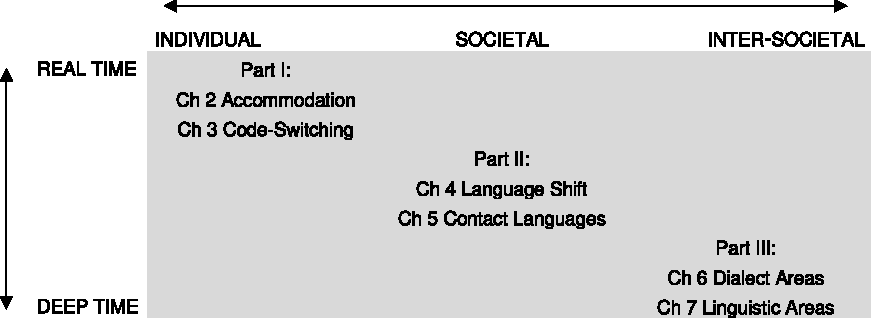
\includegraphics[width=1.0\textwidth]{Images/Structure1.png}
\end{figure}

%The dimensions of time depth (vertical axis in Figure \ref{fig-structure1}) and social scale (horizontal axis) tend to correlate. Studies focusing on the level of the individual also tend focus on short time spans (e.g. an individual conversation or at most the lifetime of an individual). Society-oriented studies may span various stretches of time, but typically not longer than a few generations. Inter-societal contact studies, finally, analyze the result of what is presumably a very long process over several generations up to thousands of years. 

%(Explain here structure of each chapter)

The remainder of this introduction will be devoted to contextualizing and explaining the approach we take in this book. Section \ref{sec-connections} discusses a number of proposals for overarching frameworks for contact linguistics. These proposals highlight potential points of commonality between different contact phenomena, but at the same time they each give a perspective on contact linguistics that is influenced by a particular subfield. In Section \ref{framework}, therefore, we propose an alternative approach. In this approach, we take a step back and look at the make-up of different research traditions within the general field of contact linguistics. Based on a unified, recurring chapter structure (see Section \ref{framework} for a discussion), specialists of each the subfields mentioned above give overviews of common practices in their respective fields, thus providing a platform for comparative contact linguistics. The final chapter of this book
%add CR
will bring the information from the different chapters together.

\subsection{Overarching frameworks for contact linguistics} \label{sec-connections}

 Several authors have proposed generalizations of language contact phenomena across the time scale and/or social scale. These studies form important pieces of the puzzle how the level of the individual in a real-time conversation connects to deep-time and society-wide historical changes due to contact. Without aiming for comprehensiveness, we discuss four illustrative models that highlight different factors in tying together contact phenomena.\footnote{These models were chosen because they are relatively recent, and because they contrast in terms of factors and phenomena that they highlight. Older, highly influential models, like \cite{Weinreich1953Languages}, \cite{thomasonetal1988language}, and \cite{van_coetsem_loan_1988} are precursors of the models presented here, and as such, their conclusions have been incorporated into the more recent models in many ways.} However, they also make clear that, even if they have points of overlap, these models regard contact effects from the perspective of a particular subdiscipline.\\
 
 \noindent
 \emph{\cite{niedzielskietal1996linguistic}: language attitudes}
 
\noindent A first example is \cite{niedzielskietal1996linguistic}, which is an attempt to apply the ideas and principles of Communication Accommodation Theory (CAT) to contact linguistics more broadly. CAT focuses on the relationship between language, social interaction, and social evaluation. According to CAT, speakers express social distance or social closeness to an interlocutor by becoming less (divergence) or more (convergence) similar in terms of their communicative behavior. For instance, speakers may start using the same linguistic expressions, adapt their speech rate to match the interlocutor's, or become more similar in their mimicry.
 CAT was first developed and tested in social psychology, primarily out of an interest in person perception and the dynamics of conversation (for details, see chapter on accommodation). 
 %insert CR accommodation
 Over the last decades, sociolinguists became interested in the theory and used the model to explain linguistic patterns within a conversation (e.g. \citealt{coupland_accommodation_1984}).
 
\cite{niedzielskietal1996linguistic} explicitly link phenomena of contact linguistics to CAT, suggesting several ways in which CAT can offer insights for longer-term contact effects. For instance, conversational research suggests that the extent to which L1 interference takes place is influenced by attitudinal factors \parencite{giles1979ethnicity}. A further application of CAT to contact linguistics discussed by \cite{niedzielskietal1996linguistic} are creoles that have developed out of pidgins. According to this idea, creoles may be seen as varieties that arise as a result of repeated mutual accommodation in situations of maximal cultural-linguistic differences between communicating groups. CAT may also contribute to the understanding of how mixed, or intertwined languages emerge, especially those that constitute secret codes. These varieties may emerge as a result of conscious divergence from interlocutors of social out-groups. Finally, CAT can also generate insights on how dialect continua and linguistic areas emerge. In areas with frequent contact between speakers of different dialects, dialect features may spread through convergence to speakers of another dialect if attitudinal factors are favorable and if speakers interact often enough. Accommodation research can shed light on the metalinguistic consciousness of specific parts of language, e.g. by investigating which linguistic parts are particularly prone to be converged on (or to be avoided) in interactions. From this point of view, accommodation research can improve our understanding of which linguistic elements are prone to be adopted by multilingual speakers, and therefore, which elements may spread in linguistic areas.\\

\noindent \emph{\cite{matras&sakel2007}: pivot matching and pattern replication}

\noindent The focus of \cite{matras&sakel2007} is to identify the mechanism that is responsible for a particular type of contact-induced effect, where ``the patterns of distribution, of grammatical and semantic meaning, and of formal-syntactic arrangement at various levels (...) are modelled on an external source." In other words: this type of contact effect does not involve the transfer of form from one language to another, but more abstract organizational and functional principles. They call this type of contact-induced change \emph{pattern borrowing}.

\textcite{matras&sakel2007} propose what they call ``pivot matching" as the mechanism involved in pattern borrowing. Their claim is that bilinguals recognize a pivotal feature  of a construction in a model language and they replicate that in a functionally equivalent construction in the replica language. What the pivot of a construction is can only be established \emph{post-hoc}: they are the elements of a construction that are copied from one language into the other (while using inherited material). \cite{matras&sakel2007} present pivot matching as a creative process whereby bilingual speakers exploit their complete bilingual repertoire to create an utterance that is formally fully monolingual, but organizationally contains elements of both languages.

The reason for pivot-matching to occur in the first place is, according to \textcite[832]{matras&sakel2007}, to ``relax to some extent the need to distinguish
between their two repertoires when planning the utterance". Pivot matching is thus first and foremost an online discourse strategy. However, if the circumstances facilitate it, these online strategies may lead to longer-term effects, thus connecting conversational contact effects to contact-induced language change, and linguistic areas. A requirement for pivot matching to have long-term effects is that the group of learners should be large enough, and the process of acquisition should never be complete. Long-term effects of pivot matching are furthermore more likely to occur in societies with relatively lax norms when it comes to grammatical rules, so that pivot matching is not corrected.

Social constraints, for instance a social policy against mixing of language matter (phonetic substance), as e.g. in the Vaupés in Amazonia (see chapter on linguistic areas) may also facilitate or promote pivot matching, increasing the potential of long-term effects.
%add CR

Matter borrowing (over pattern borrowing) may also be influenced by structural-linguistic factors. These have to do with the resistance to or unlikelihood of matter borrowing for some highly entrenched linguistic elements such as inflectional morphology. More generally speaking, some constructions favor matter borrowing, others pattern borrowing, and yet others seem to have no clear preference. Linguistic constraints may also be relative, subject to the inventory of linguistic elements in the replica language that can be exploited for pivot matching in a particular construction. Other forces at work mentioned by \cite{matras&sakel2007} are the fact that some features of constructions appear to be essential and thus immune to modification, and phonetic similarity.\\

\noindent \emph{\cite{myersetal2009universal}: lexicon versus structure}

\noindent A different overarching model is presented in \cite{myersetal2009universal}. The central assumption of the model, which was originally developed to tackle certain types of code-switching phenomena, is that contact phenomena display non-random patterns in that they follow the \emph{structural patterns} of one language, inserting \emph{content} from other languages into this structural frame (the Uniform Structure Principle). The language that supplies the structure (termed the matrix) is referred to as the \emph{Matrix Language}, the language that supplies content material that is inserted into the matrix is referred to as the \emph{Embedded Language}.

The second major part of the model is an elaboration of what is structure (part of the matrix) and what is content. Four types of morphemes\footnote{The term ``morpheme" is used in a generalized sense to refer to abstract entries or features and their surface realisations.} are distinguished: 

%present a general model of language contact, which was originally developed as a model of code switching with relevance for other types of contact phenomena. This generalized model is driven by the \textit{Uniform Structure Principle}, which says that code switching in bilingual speech (and, as we will see, in other contact phenomena) displays non-random patterns in that it follows the structure of one of the languages, inserting content from other languages into this structural frame. 

%This general principle is translated into a model developed for code switching, called the \textit{Matrix Language Frame} model (MLF). In this model it is claimed that code-switched utterances involve a \textit{matrix language} supplying linearization principles and more system-like morphemes, and an \textit{embedded language} supplying the more content-like morphemes. Three types of system morphemes are distinguished: 
\begin{itemize}
\itemsep0em 
    \item \textsc{Content morphemes}: conceptually salient material that receives or assigns thematic roles (i.e. argument roles such as agent, patient, beneficiary, etc.).
    \item \textsc{Early system morphemes}: conceptually salient building blocks of phrase structures, which do not receive or assign thematic roles (e.g. articles, derivational affixes, verbal particles).
    \item \textsc{Bridge late system morphemes}: Structurally assigned material that connects (builds bridges) between elements of a constituent, and that depends on information within its constituent (e.g. markers of possession, partitive markers, expletives).
    \item \textsc{Outsider late system morphemes}: Structurally assigned material that depends on information outside of the immediate constituent (e.g. subject-verb agreement, case markers).
\end{itemize}

The main idea is that the four morpheme types (content morphemes and the three system morpheme types) can be ordered as to how likely it is that they come from the embedded or matrix language in a mixed utterance (see Table \ref{tab-ms-model}). 

\begin{table}
\small
\caption{Morpheme types and source languages}  
\label{tab-ms-model}
 \begin{tabular}{lccr}
 %l{2cm}  l{2cm}  r{2cm} r{2cm}} 
  \lsptoprule
 embedded language & & & matrix language\\ 
  \midrule
  content morphemes & early system morphemes & late bridges & late outsiders\\ 
   \lspbottomrule
 \end{tabular}
\end{table}

The authors connect this to a psycholinguistic language production model proposed in \cite{levelt1989speaking} in which (among other things) a distinction is made between selecting items (lemmas with associated forms) from a mental lexicon, and subsequently generating a grammatical context for these items.

Myers Scotton and Jake's claim is that content morphemes and early system morphemes are part of the mental lexicon, whereas late bridges and late outsiders are generated as part of the grammatical context. In this sense, the model proposed by \cite{myersetal2009universal} stresses both linguistic structure and language processing as important factors in explaining contact patterns, at least in code switching. 

According to \cite[291]{myers1998way} ``the same structural processes figure in all forms of bilingual speech, from code switching to interlanguage in second language acquisition, to language attrition, to mixed languages or pidgins and creoles". In other words: Myers Scotton explicitly links individual, real-time behavior (code-switching) to historical processes at the societal level (language attrition, contact language formation), suggesting that they can be tackled by one and the same model (see e.g. \citealt{myers1998way} for an elaboration).\\

%\cite{myers1998way} is an elaboration of how the MLF model deals with language attrition.\footnote{Myers Scotton stresses that the MLF model cannot deal with contact phenomena that do not involve structural modifications in the participating languages.} Using the basic ingredients discussed above (the ML frame and the morpheme types), she introduces two functional extensions: since ML assignment is dynamic, there can be a ML \emph{turnover}, essentially a switch of roles where the ML becomes the EL, and another variety takes over as ML. Second, MLs can be \emph{composite}, and this is, Myers Scotton claims, what often happens in the process of ML turnover. ML turnover and composite ML can, in Myers Scotton's view, explain some patterns found in community-level, longer-term processes such as "advanced stages of convergence, structural borrowing, or attrition" \citep[300]{myers1998way}.

%An ML turnover, in this view, results from situations where there is widespread intra-sentential code-switching or convergence, a shift occurs in the socio-political balance. Myers Scotton discusses three possible outcomes of ML turnover.

%\begin{enumerate}
    %\item ML turnover is arrested, but traces of the competing ML remain leading to situations that have been termed "structural borrowing".
    %\item A composite ML is fossilized (this can happen at different stages of the turnover process) which may result in a mixed or intertwined language.
    %\item The turnover goes to completion, which can subsequently result in language attrition of the old ML and even complete shift towards the new ML.
%\end{enumerate}

\noindent \emph{\cite{muysken2013language}: social and linguistic asymmetries}

\noindent A framework for explaining language contact phenomena based on certain asymmetries between aspects of the first language (L1) and the second languages (L2) of a group of bilinguals is presented in \cite{muysken2013language}. He introduces four general bilingual ``optimization strategies", which are typically applied by bilingual speakers in different sociolinguistic circumstances. These optimization strategies and their brief descriptions are given in Table \ref{tab-muysken_OS}; the numbers are indices for later referral in the running text.

\begin{table}
\caption{Four bilingual optimization strategies}  
\label{tab-muysken_OS}
%\resizebox{\textwidth}{!}{
 \begin{tabular}{lll} 
  \lsptoprule
 Nr. & Shorthand & Description \\ 
  \midrule
  1 & L1 & Maximize structural coherence of the first language \\
  2 & L2 & Maximize structural coherence of the second language\\
  3 & L1/L2 & Match between L1 and L2 patterns where possible\\
  4 & UP & Rely on universal principles of language processing\\
   \lspbottomrule
 \end{tabular}
 %}
\end{table}

\cite{muysken2013language} argues that these four generalized strategies are applied in different ways depending on the circumstances, leading to different outcomes, both in conversations and in patterns that are the result of sustained contact over time. Strategy 1 tends to occur in situations where L1 has high prestige and/or speakers of L1 have low proficiency in L2, and/or limited access to L2. The second strategy is often employed in opposite circumstances, i.e. where L2 has high prestige and/or proficiency in L2 is high and/or there are large numbers of L2 speakers. Strategy 3 is prototypically connected to situations of low normativity (i.e. where there is more social tolerance for using different structures), but also to situations where L1 and L2 are lexically and/or typologically similar to each other. The final strategy is found in situations where the social and linguistic distance between the L1 and L2 groups is large, and/or the contact period brief.

Muysken's model is best illustrated by looking at code-switching, for which it seems to be developed in most detail. Based on earlier work \parencite{muysken2000}, he distinguishes four different patterns in code switching (Table \ref{tab-muysken_CS}:

\begin{table}
\caption{Four bilingual optimization strategies}  
\label{tab-muysken_CS}
 \begin{tabular}{p{2.6cm} p{9cm}} 
  \lsptoprule
 Type & Description \\ 
  \midrule
 \textsc{Insertion} & One of the languages (L1) is used as the matrix language, and the other (L2) as the embedded one.\\
    \textsc{Congruent lexicalization} & Elements from either language are used in constructions that are (partly) shared by the languages.\\
    \textsc{Alternation} & The use of fragments of L1 and L2 in succession within a sentence, regulated by universal combinatory possibilities.\\
    \textsc{Backflagging} & Insertion of material from the heritage language (L1) in an otherwise L2 discourse.\\
\lspbottomrule
 \end{tabular}
\end{table}

He connects each of these strategies to one of the optimization strategies mentioned in Table \ref{tab-muysken_OS}. Insertion is considered to be the result of strategy L1, because it inserts content elements from L2 in an otherwise L1 structural environment. As such, the structural coherence of L1 is maximized (kept intact). Congruent lexicalization results from the L1/L2 strategy, in that it is an attempt to combine elements from both languages that are partly shared. Alternation can be connected to the strategy UP to the extent that the way in which elements from both languages are combined follows universal principles. Backflagging, finally, results from the L2 strategy, because the structural integrity of L2 is respected, and elements of the heritage language are inserted. This is the mirror image of insertion.

\cite{muysken2013language} explicitly claims that these strategies are responsible for many different contact phenomena at different social scales and time depths. It is beyond the scope of this introduction to discuss this in detail (for this the reader is referred to \citealt{muysken2013language}, but the model and its interpretations for other contact phenomena relevant to this book is given in Table \ref{tab-muysken}).

\begin{table}
\caption{Bilingual optimization strategies and contact phenomena}  
\label{tab-muysken}
%\resizebox{\textwidth}{!}{
 \begin{tabular}{p{1cm} p{2.5cm} p{3cm} p{4cm}} 
  \lsptoprule
 & code-switching & contact languages & contact-induced change \\ 
  \midrule
  L1 & insertion & relexified languages, L1-oriented pidgins & borrowed forms adapt to L1 functionality \\
  L2 & backflagging & lexifier-oriented contact languages,  & transfer, substrate\\
  L1/L2 & congruent lexicalization & compromise contact languages & merging aspects from both languages, convergence\\
  UP & alternation & bioprogram & simplification, adopting unmarked structures\\
   \lspbottomrule
 \end{tabular}
 %}
\end{table}

Of relevance to the present book is that Muysken identifies a set of factors that are involved in the choice of optimization strategy \citep[726]{muysken2013language}. We come back to the issue of factors in the next section and at various points in the book.

\begin{itemize}
\itemsep-0.4em 
    \item similarity factors (lexical and typological);
    \item prestige and status factors;
    \item proficiency factors;
     \item contact factor (group size, network type);
    \item time factors (of contact period);
    \item attitudinal factors (low normativity, political
distance).
\end{itemize}

%Muysken connects these four patterns in CS to the four bilingual optimization strategies (and associated social circumstances, where insertion is connected to optimization strategy 1 above (L1), backflagging is associated with the second strategy (L2), congruent lexicalization is connected to strategy 3 (L1/L2), and alternation to strategy 4 (UP). 

%Muysken extends this explanatory framework to longer-term contact phenomena, such the formation of contact languages (creoles, pidgins, mixed languages, ethnolects), and more generally contact-induced change that eventually may lead to language loss and to linguistic areas.

%With respect to contact languages %add cross reference
%Muysken considers pidgins, creole languages, and mixed languages. For each of these, he distinguishes four subtypes that correspond to one of the optimization strategies.

%L1-strategy creole languages arise in situations where many speakers of one or a few of the L1s are present leading to strong substrate influence of these L1s on the creole language. Muysken terms this relexification and mentions Saramaccan as an example. L2-strategy Creoles arise in situations of relative balance between the L2 speakers and the speakers of a single L1 may lead to a Creole language that shows convergence between the systems. Possible examples mentioned by Muysken are Berbice Dutch Creole and Senegal Portuguese Creole. UP-strategies, referred to as "bioprogram" by \cite{bickerton_roots_1981} may be resorted to in situations where there are many L1s present, and the L2 is not very accessible. Hawaiian Creole may show a number of these structures. Strong presence of the L2 at the time of Creole formation may lead to Creoles that are close to the European lexifier language, coming close to language shift. French Reunión Creole is an example of this type of Creole.

%Parallel subdivisions exist to some extent for pidgins and mixed languages. L1-oriented pidgins, like Ndyuka-Trio Pidgin and Pidgin Delaware, where a local population came in contact with newcomers, leading to pidgins that are predominantly based on the resident group's language. L1-oriented mixed languages (like Media Lengua) arise in situations of a limited presence of the lexifier languages, and incorporate L2 elements into an otherwise L1 grammatical and phonological frame.

%L2-oriented pidgins are simplified versions of a target languages that arise as the result of second language acquisition in situations of large social distances between immigrant communities and lexifier communities. In L2-oriented mixed languages the lexifier language contributes important chunks of grammatical structure resulting from language shift. An example is Mednyj (or Copper Island) Aleut. 

%Generally speaking pidgins and mixed languages may contain several UP-based elements that lack in the unmixed versions of the contributing languages. Muysken mentions the use of reduplication in Media Lengua and Callahuaya, not present in the contributing languages.

%Compromise versions of pidgins and mixed languages have mixed lexicons and mixed grammatical structures with both L1 and L2 languages contributing. This may arise in situation of more equal status of the L1 and L2 languages.

%Contact-induced change can also be classified according to the model proposed by Muysken. L1-oriented change involves situations where material or patterns from the L2 are blended into a maintained L1 structure. This is for instance the case when the form of an affix from L2 is borrowed, but taking on the meaning of an existing native affix, or the adjustment of loan phones to fit the L1 system.

%L2-oriented change involves e.g. the spread of L2 morphemes to native words, the wholesale adoption of grammatical patterns or lexical items, foreign phonemes unadapted to L1 structures. 

%Much has been said about simplification effects of contact (e.g. \citealt{kusters_linguistic_2003,miestamo2008language,Sampsonetal2009Language,Lupyanetal2010Language,Trudgill:2011}). It is not entirely clear how and/or to what extent this interacts with universal principles, but very generally speaking, simpler structures are easier to process. Contact-induced change governed by universal principles includes loss or reduction of word order variations, morphosyntactic features, and of marked elements in phoneme inventories or marked syllable structures.


\noindent What these models have in common is that they point to phenomena that recur in different contact-related situations, from language mixing patterns in real-time bilingual conversations to deep-time contact-effects that have spread through entire communities. They differ in what they see as crucial factors contributing to these recurring patterns. Where \cite{niedzielskietal1996linguistic} highlight the importance of attitudinal factors, \cite{matras&sakel2007} focus on language processing, Myers Scotton and Jake's \citeyear{myersetal2009universal} model gives central stage to linguistic structure and the lexicon-structure distinction, and Muysken's model focuses on optimal communication strategies of bilinguals given certain (a)symmetries in the circumstances (taking into account aspects such as language access, power relations, typological distance). These models suggest that contact phenomena from individual conversations to Sprachbund phenomena are connected, but they also highlight that several perspectives on the factors contributing to these connections are possible. This makes it hard to bring all these different perspectives together. One of the reasons for the different focal points may be that the authors in the models presented above look at different contact effects through a particular prism (whether that is an accommodation prism, a code-switching prism, a convergence prism, or a symmetry prism). 

\subsection{The approach of the present book} \label{framework}

The present book differs from these (and other) approaches in two main respects. First, this is a multi-authored effort that involves specialists from the different subdisciplines that are central to this book. This ensures that each subdiscipline is treated even-handedly. Second, rather than focusing only on what the implications of the results of subdiscipline A are for subdiscipline B, it takes a further step back and compares the research traditions of each subdiscipline. 

While Figure 1 suggests that the phenomena described in the book are maximally different from each other, a more detailed overview reveals that each of the subfields addressed in this book often has a broader range and spillovers with neighboring fields, as shown in Figure \ref{fig-structure2}, where numbers between brackets refer to chapters.

\begin{figure}[h]
\caption{The relationship between each of the book's topics with the two dimensions, time and social scale} \label{fig-structure2}
\centering
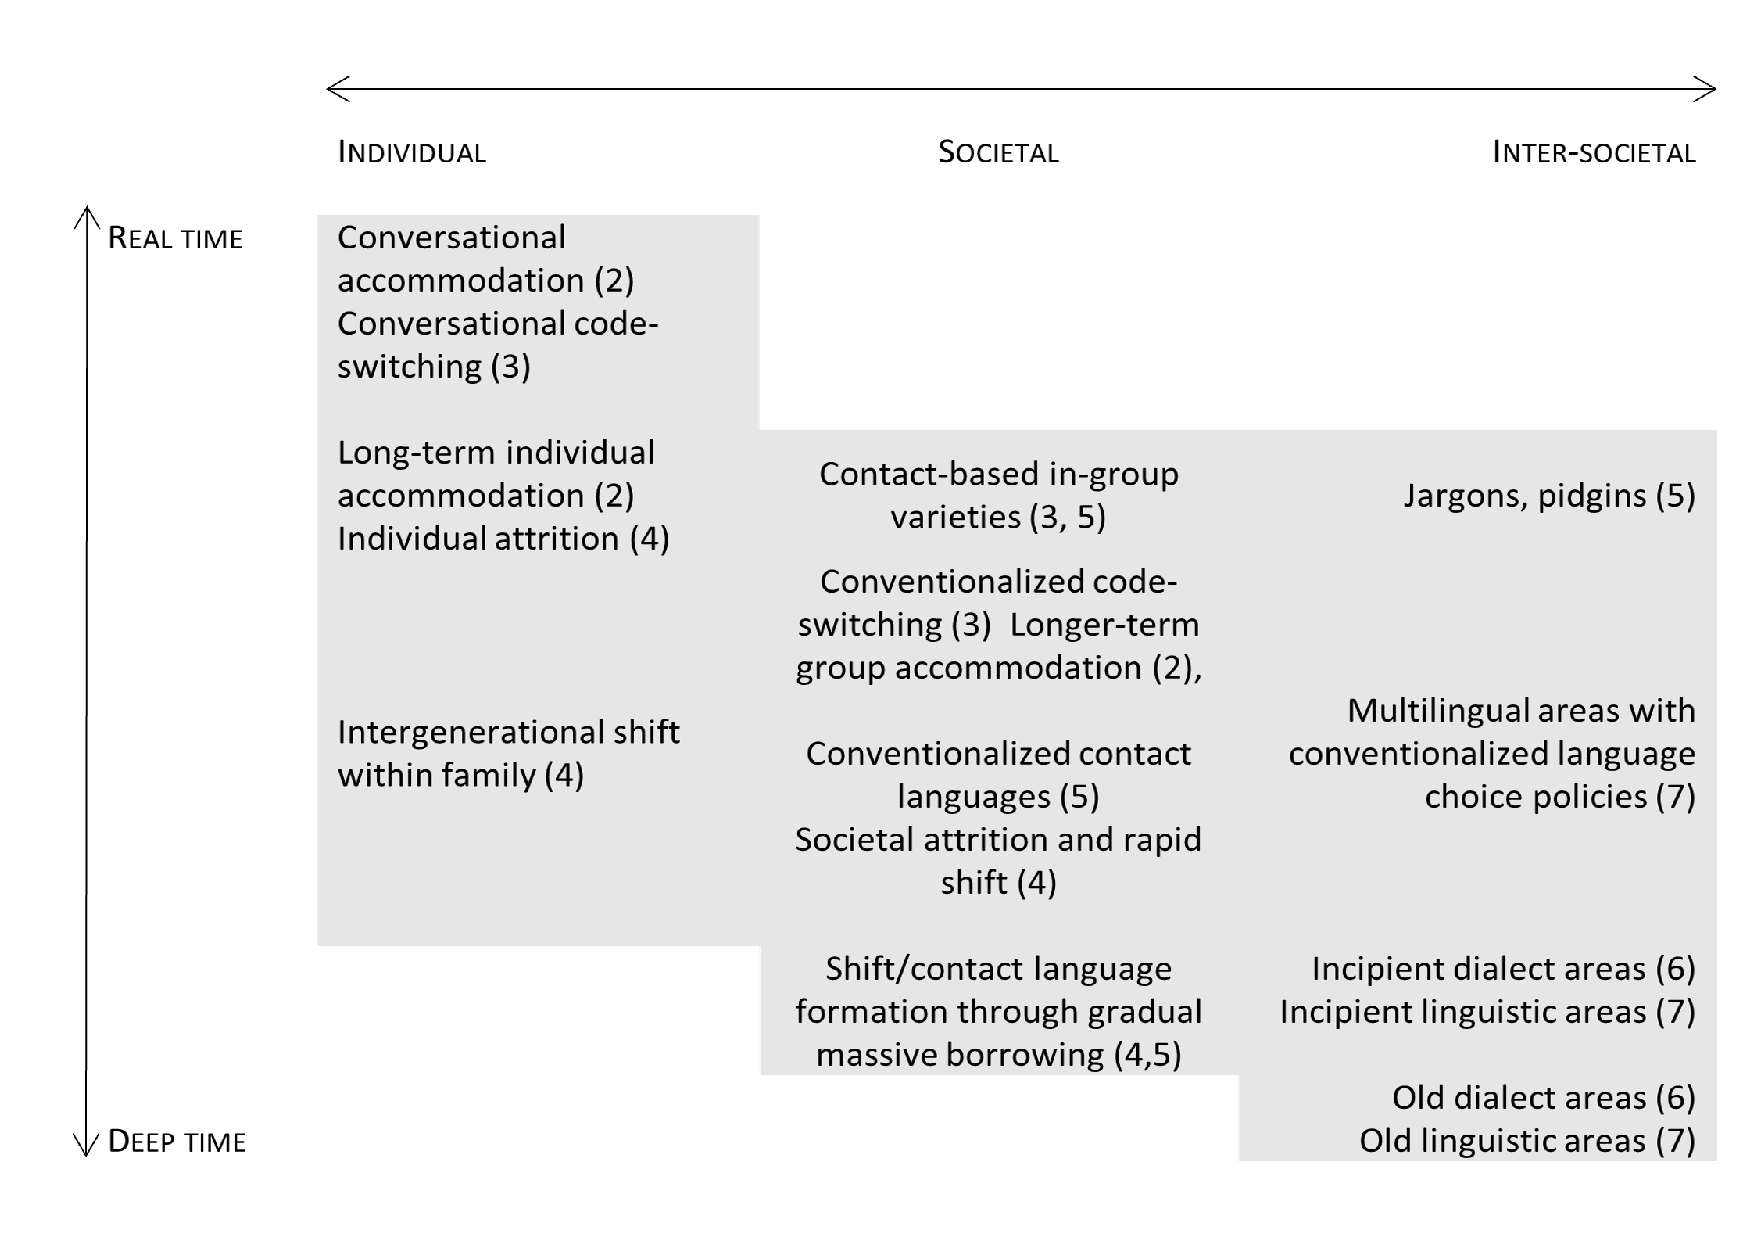
\includegraphics[width=1.0\textwidth]{Images/Structure2.png}
\end{figure}

These overlaps allow for more in-depth comparisons between different phenomena across the subfields and for a more precise assessment of the effects of time, social scale, and of course research practices.

\subsubsection*{Approaches}
The approaches used in each subfield to explain their phenomena of interest exhibit further potential for comparison across subfields. We focus especially on the way in which the subfields model their predictions on the basis of empirically available data. Studies concerned with conversational interactions model the effects of short-term contact-induced effects into deeper time, predicting how conversational patterns may lead to contact-induced change (see in particular \cite{niedzielskietal1996linguistic} on how patterns of accommodation in conversations may lead to patterns of convergence, or \cite{myers2008language} on how patterns found in conversational code switching recur in all products of language contact). Areal studies often only have the present-day linguistic patterns to go on, and therefore their models seek to reconstruct the past scenario(s) that gave rise to the present situation \parencite[see e.g.][]{muysken2010scenarios, Nichols2003Diversity}. Modelling in the study of contact varieties and language shift may go both ways: predicting what scenarios will lead to contact varieties or language shift or to contact varieties, or filling the gaps of the often incomplete historical record on the basis of the synchronic (language) data.

Therefore, a comparison of models and empirical evidence across subfields can be mutually beneficial: interactional research can test their predictions by looking at areal patterns and patterns in contact varieties and language loss, and the study of contact varieties, language shift, and areal linguistics can be informed from accommodation or code-switching studies about possible outcomes of individual interactions.


\subsubsection*{Linguistic patterns}
All of the subfields discussed in this book are invested in the question ``What type of linguistic patterns do we observe?" Because all approaches try to generalize across the different patterns found for the particular phenomenon in question (code-switching patterns, typical Creole structure, features prone to diffuse, etc.) they form a basis for direct comparison: to what extent do we find similar patterns in, for instance, code-switching and mixed languages, in dialect areas and linguistic areas, and in accommodation and language shift?



\subsubsection*{Factors}
In addition, all approaches discuss factors that may influence the observed outcomes. Some of these factors relate to characteristics of individuals (e.g. age, attitudes) or the speech situation (e.g. conversational topic), others relate to the varieties involved (e.g. typological distance), to societal parameters (e.g. subsistence strategies, language ideologies), or to the geographical circumstances (e.g. topographical elements that facilitate or impede contact, (travel) distance). Despite the fact that conversational approaches put more emphasis on characteristics of the individual and the speech situation, and areal approaches on geographical factors, there is an overlap in particular in the societal and linguistic factors involved, allowing for relatively direct comparison.



\subsubsection*{Further dimensions}

It goes without saying that contact linguistics operates on many more dimensions than social scale and time depth, and, in this respect, we do not aim for completeness in the book. However, some further dimensions do play a role, which for their part allow for other connections between subfields. An obvious opposition between dialect areas and linguistic areas is genealogical relatedness (which is usually associated with typological distance). This opposition partly echoes the opposition between accommodation and code-switching, phenomena that are usually observed between closely related or distantly/unrelated languages, respectively. A second opposition worth mentioning is between contact-induced language birth and language death, which figures in Part II of the book. There may be many sociolinguistic processes giving rise to the formation of linguistic areas, including language shift, societal L2 effects, and language mixing, all of which are discussed in the chapters on language shift and contact varieties. The opposition birth–death of varieties, finally, may be the societal outcome of accommodation or code-switching.


\subsection{The organization of this book}

Given these points of interest, we structure the book in such a way that  the potential areas of overlap are maximally highlighted. Each chapter has the same basic structure, which looks as follows.

\begin{enumerate}
\item Introduction

Definition of the phenomenon in question as well as of important concepts in the subfield, its main research questions, and a discussion of how the subfield relates to the others in the book.

\item Approaches

A discussion of the most important models and methods used per subfield.

\item Linguistic patterns

An overview of the linguistic patterns observed (outcomes) for each of the subfields discussed in the book that require an explanation.

\item Factors

A discussion of the factors shown or assumed to be relevant to explain the patterns and processes at the core of the subfield.

\item Conclusion and outlook

Overview of the main conclusions of the chapter, identifying major gaps in the research domain, and a discussion of possible future directions, with the aim of bridging the gap between the subfields.
\end{enumerate}

This set-up allows for a systematic comparison across the disciplines. In the final chapter we take such a comparative perspective and formulate our conclusions about the unity of the field of contact linguistics, and possibilities for cross-overs, opening up new perspectives for the future.

\printbibliography[heading=subbibliography,notkeyword=this]

\end{document}
